\documentclass{article}

\usepackage[hmargin=20mm, vmargin=25mm]{geometry}
\usepackage{parskip}
\usepackage{amsmath}
\usepackage{graphicx}
\graphicspath{ {../figures/} }
\begin{document}
\title{Data, Estimation and Inference Report}
\author{Ben Ellis}
\date{\today}
\maketitle

% Describe the data that we are trying to fit and its patterns
This report considers data from a sensor measuring tide height.
The sensor often fails to transmit readings due to severe weather, and 
hence we here try to interpolate from the data available.

The readings from the sensor and the true tide heights over the period 
considered are shown in Figure \ref{fig:scatter}. 

\begin{figure}
    \centering
    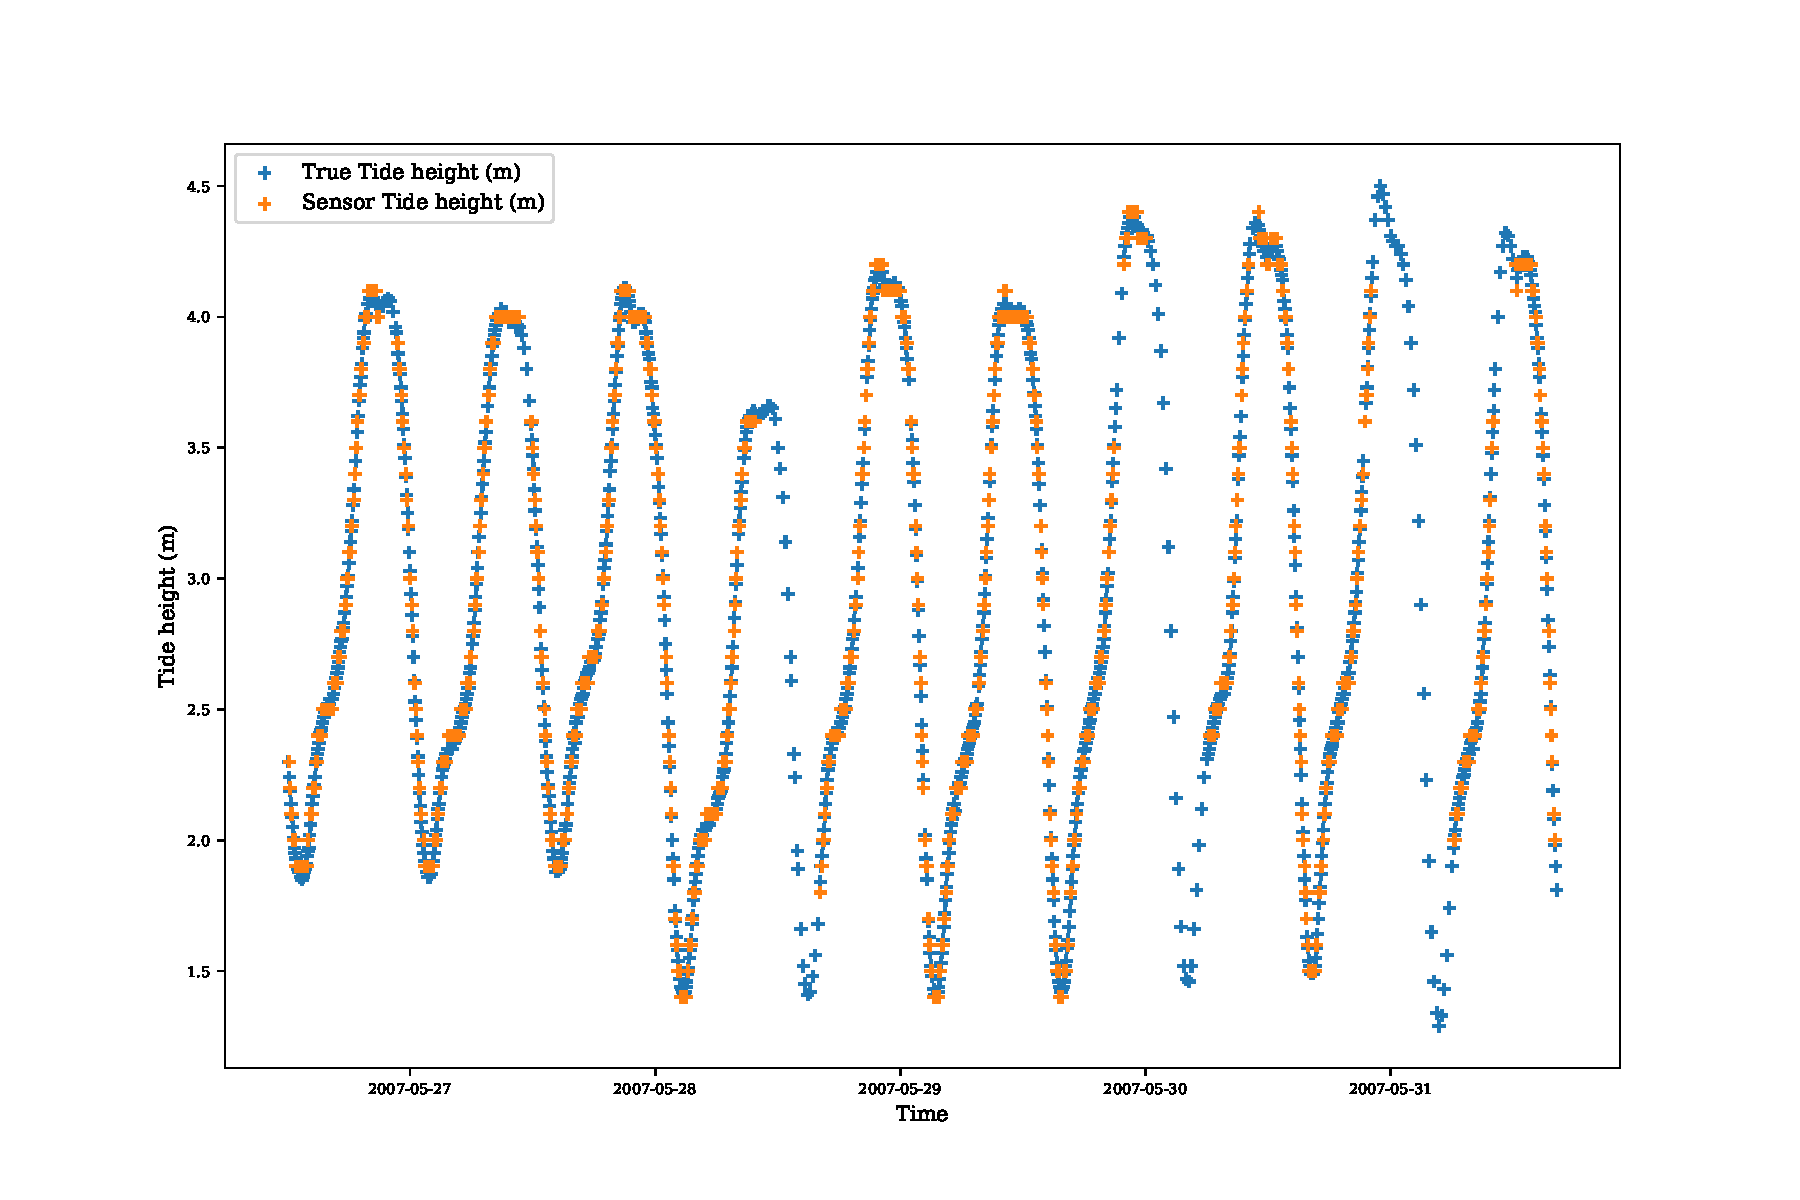
\includegraphics[width=\textwidth]{sensor_scatter}
    \caption{Scatter plot of the data obtained by the sensor and the true tide height}
    \label{fig:scatter}
\end{figure}

This data exhibits a few interesting patterns:
\begin{itemize}
    \item As we would expect, the tide height is periodic with a period of roughly 12 hours.
    \item There are a few notable periods where data are entirely missing.
    \item Although data are missing, observed readings show relatively little noise.
\end{itemize}

The regular structure of the data suggests that we could use Gaussian Processes to interpolate.

\section*{Gaussian Processes}

A Gaussian process $f(\mathbf{x}) \sim \mathcal{GP}(m(\mathbf{x}), K(\mathbf{x}, \mathbf{x}))$ is a collection
of random variables, any finite collection of which is Gaussian distributed. More specifically, any finite collection 
of function values $f(\mathbf{x}_1), \dots, f(\mathbf{x}_n)$ will have the distribution
\[
    \begin{bmatrix}
        f(\mathbf{x}_1) \\
        f(\mathbf{x}_2) \\
        \vdots \\
        f(\mathbf{x}_n)
    \end{bmatrix} \sim 
    \mathcal{N}\begin{pmatrix}
        \begin{bmatrix}
            m(\mathbf{x}_1) \\
            m(\mathbf{x}_2) \\
            \vdots \\
            m(\mathbf{x}_n)
        \end{bmatrix}, 
        \begin{bmatrix}
            K(\mathbf{x}_1, \mathbf{x}_1) & K(\mathbf{x}_1, \mathbf{x}_2) & \dots & K(\mathbf{x}_1, \mathbf{x}_n) \\
            K(\mathbf{x}_2, \mathbf{x}_1) & K(\mathbf{x}_2, \mathbf{x}_2) & \dots & K(\mathbf{x}_2, \mathbf{x}_n) \\
            \vdots & \vdots & \ddots & \vdots \\
            K(\mathbf{x}_n, \mathbf{x}_1) & K(\mathbf{x}_n, \mathbf{x}_2) & \dots & K(\mathbf{x}_n, \mathbf{x}_n)
        \end{bmatrix}
    \end{pmatrix}
\]
Here $m$ is a function which gives the value of the mean of the gaussian at its input, and $K$ is a kernel function which given
inputs $\mathbf{x}_i$ and $\mathbf{x}_j$ computes the entry in the covariance matrix $\Sigma_{ij}$. This means that for any point
$\mathbf{x}_{\star}$ the Gaussian process induces a Gaussian distribution of the possible function values $f(\mathbf{x}_{\star}$.
This is shown for a simple linear case in Figure \ref{fig:func_distribution}. And things stuff
\begin{figure}
\centering
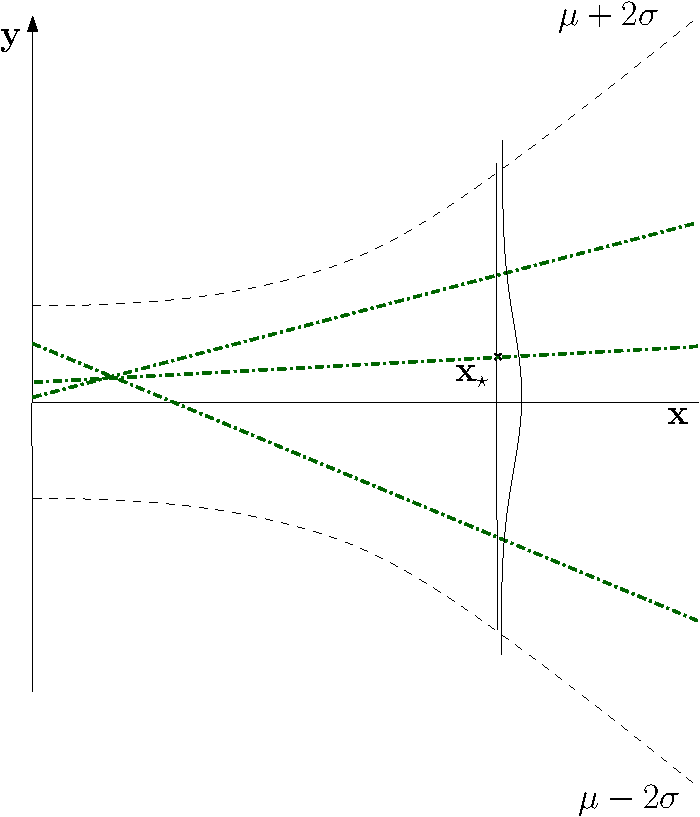
\includegraphics[width=0.5\textwidth]{function_distribution_cropped}
\caption{Diagram illustrating a Gaussian distribution over function values at $\mathbf{x}_{\star}$. Some simple functions drawn
from the distribution are shown in dark green.}
\label{fig:func_distribution}
\end{figure}
% Why use gaussian process here? 
% Looks like a fairly regular function so limited expressivity not a problem
% Describe gaussian processes 
% Describe the marginal likelihood.
% Talk about 0 mean assumption and normalisation of data
% Talk about kernel choice. 



\end{document}

